Consider a user request which defines a start period $T_0=[T_{0i}, T_{0f}]$,
a start city, $v_0$, a return city $v_{n+1}$, and a list of cities to be visited,
$V$, where upon visiting each city $i$ $\in$ $V$, a waiting periof of $d_i$ days is necessary.

The steps necessary to construct a random solution to this request are illustrated in figure \ref{fig:random_solution},
and can be summarized as follows. Start by setting the initial time, $t \in T_0$, and the current node, $v_c = v_0$.
If there are no nodes to visit, that is, if $V = \{\}$, a solution if defined by the flight $a_{v_0, v_{n+1}}^{t}$.
Otherwise, select a random city, $v_i \in V$,
and extend the solution with the flight $a_{v_c, v_{i}}^{t}$. Follow this with the update of $t = t + d_i$,
remove the selected node $v_i$ from $V$, and set it as the current node.
Repeat this process untill all nodes are visited, and conclude by closing the tour.

The described process may start immediatly after receiving a request,
because it does not require the information relative to the arcs of the problem.
Instead, it generates a completly random solution, composed of several flights,
whose information is not yet known. 
Thus, this solution is passed to the Data Management System, which calls a third-party API 
to request the relevant information. If the number of flights which constitute the solution is lower than 9,
this information can be obtained with a single HTTP request to the API. Otherwise, the number of necessary requests 
is given by, approximately, $N/10 + 1$, where $N$ is the number of necessary flights.


% \begin{enumerate}
%   \item set an initial empty solution, $s$ = ();
%   \item select a start date, $t_0 \in T_0$;
%   \item define the current node $v_c = v_0$, and the current time $t = t_0$;
%   \item if V = $\{\}$ go to step 9);
%   \item select a random city $v_i \in V$;
%   \item extend the solution $s$ with the arc $a_{v_c, v_i}^{t}$;
%   \item increment time: $t = t + d_i$, and set current node $v_a = v_i$, remove $v_i$ from $V$;
%   \item go to step 4);
%   \item extend the solution $s$ with the arc $a_{v_c, v_{n+1}}^{t}$;
% \end{enumerate}

\begin{figure}[htpb]
  \centering
  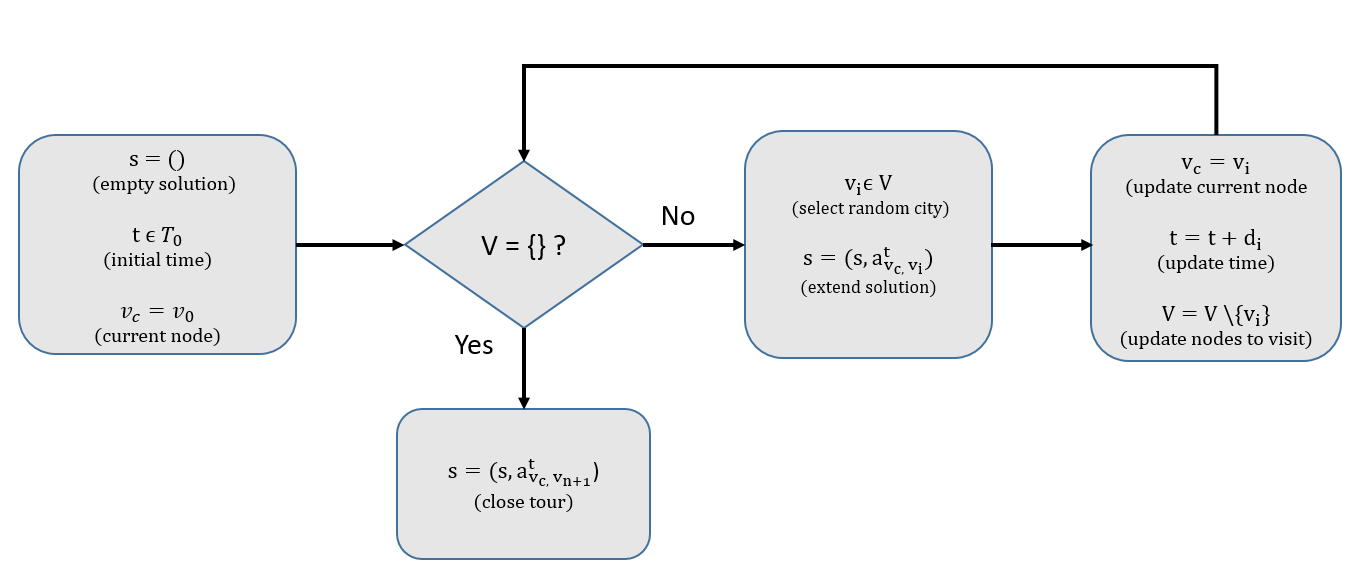
\includegraphics[width=\textwidth]{Figures/system_implementation/random_solution.png}
  \caption{Steps to generate a random solution to a user request.}
  \label{fig:random_solution}  
\end{figure}

While the random solution generation may start immediatly after receiving a request,
the nearest neighbour heuristic relies on a complete cost matrix,
and so can not be initiated before collecting all the information necessary.
The nearest neighbour algorithm is closely related to the process described in figure \ref{fig:random_solution},
however, instead of selecting a random node $i \in V$,
this node is selected according to its cost. At any point of the process, there is a \textit{current} node and time,
which can be used to determine all the possible solution components (arcs), where the one with the lowest cost is selected.
Furthermore, if the start time of the request is given by a time window,
the illustrated process can be repeated for all allowable start dates.






